%!TEX root = ../master.tex
\chapter{Design}\label{ch:design}
\todo{This part needs rework. Write after chapter is done.}
This chapter will cover the design iterations and the decisions that were made. 

\section{Initial brainstorm}\label{sec:initialbrianstom}
The initial brainstorm consisted of two brainstorms that was chained together. The starting point of the first brainstorm was the point "Image to sound" and the second brainstorms starting point was "Filters". 

\begin{figure}[!h] 
\centering
\includegraphics[width=1\textwidth]{initialbrainstorm}
\caption{\label{fig:initialbrainstorm} The initial brainstorm. Orange bubbles indicates the starting points, the blue bubbles indicate the chosen topics within the "Image to sound" brainstorm and the red bubbles are the chosen filter and filter methods within "Filters" brainstorm.}
\end{figure}

All the points from "Image to sound" are a mixture of manipulative image processing factors and image capturing methods. 
The points expanding from "Filters" relates to tools the user can apply to the audio created from the image. 
"Filters" branches out to the point called "Different Filters" which lists various common filters that may be applied to the audio. It also branches out to the point called "Controls". Controlling multiple filters can relate to an equalizer. \todo{sæt lidt mere på sætningien}
Since it is stated in the final problem statement that it is a requirement to be able to control the filters, the point "Controls" is essential in the brainstorm. From "Controls", different methods of controlling filters were considered, and from these "Toggle all filters", "Intensity of filter", "Multiple filters at once" and "Peripheral devices to adjust intensity" were chosen for the design.

Based on the final problem statement the design team chose to narrow down the brainstorm, which resulted in working with an RGB image that can be replaced at any time. Then bandpass, comb and high shelf filters are applied, and the user is able to apply these individually or at the same time with the possibility to change the intensity of the filters by using peripheral devices. 
The reason for choosing the specific filters is the theory behind them. Many of the listed filters are similar in the way they work, but the chosen filters differentiate between each other in the way they alter the sound.


\section{Conceptual model}\label{sec:concept}
This project will work with audiolisation of an image. The initial design is focused on the conversion of images into an audio signal. \todo{beskriv gerne mere i dybden}Each pixel has a value for each RGB colour channel that can be converted into a range that fits the human hearing, which is defined to be between 20 to 20.000Hz \todo{insert reference with human hearing range definition}. The output of this operation can then be manipulated by audio processing filters \todo{insert reference}.

The concept includes a control interface in the artefact. It allows the user to have control over the output in real time, as the control interface will change how the filter effects will modify the image-created audio. This gives the user agency of how the output will sound. To allow the user to create even more unique sounds, multiple filter can be applied simultaneously. This allows for a wide range of artistic expression, as the user will have control over the audio output.

\section{Storyboard}
\begin{figure}[!h] 
\centering
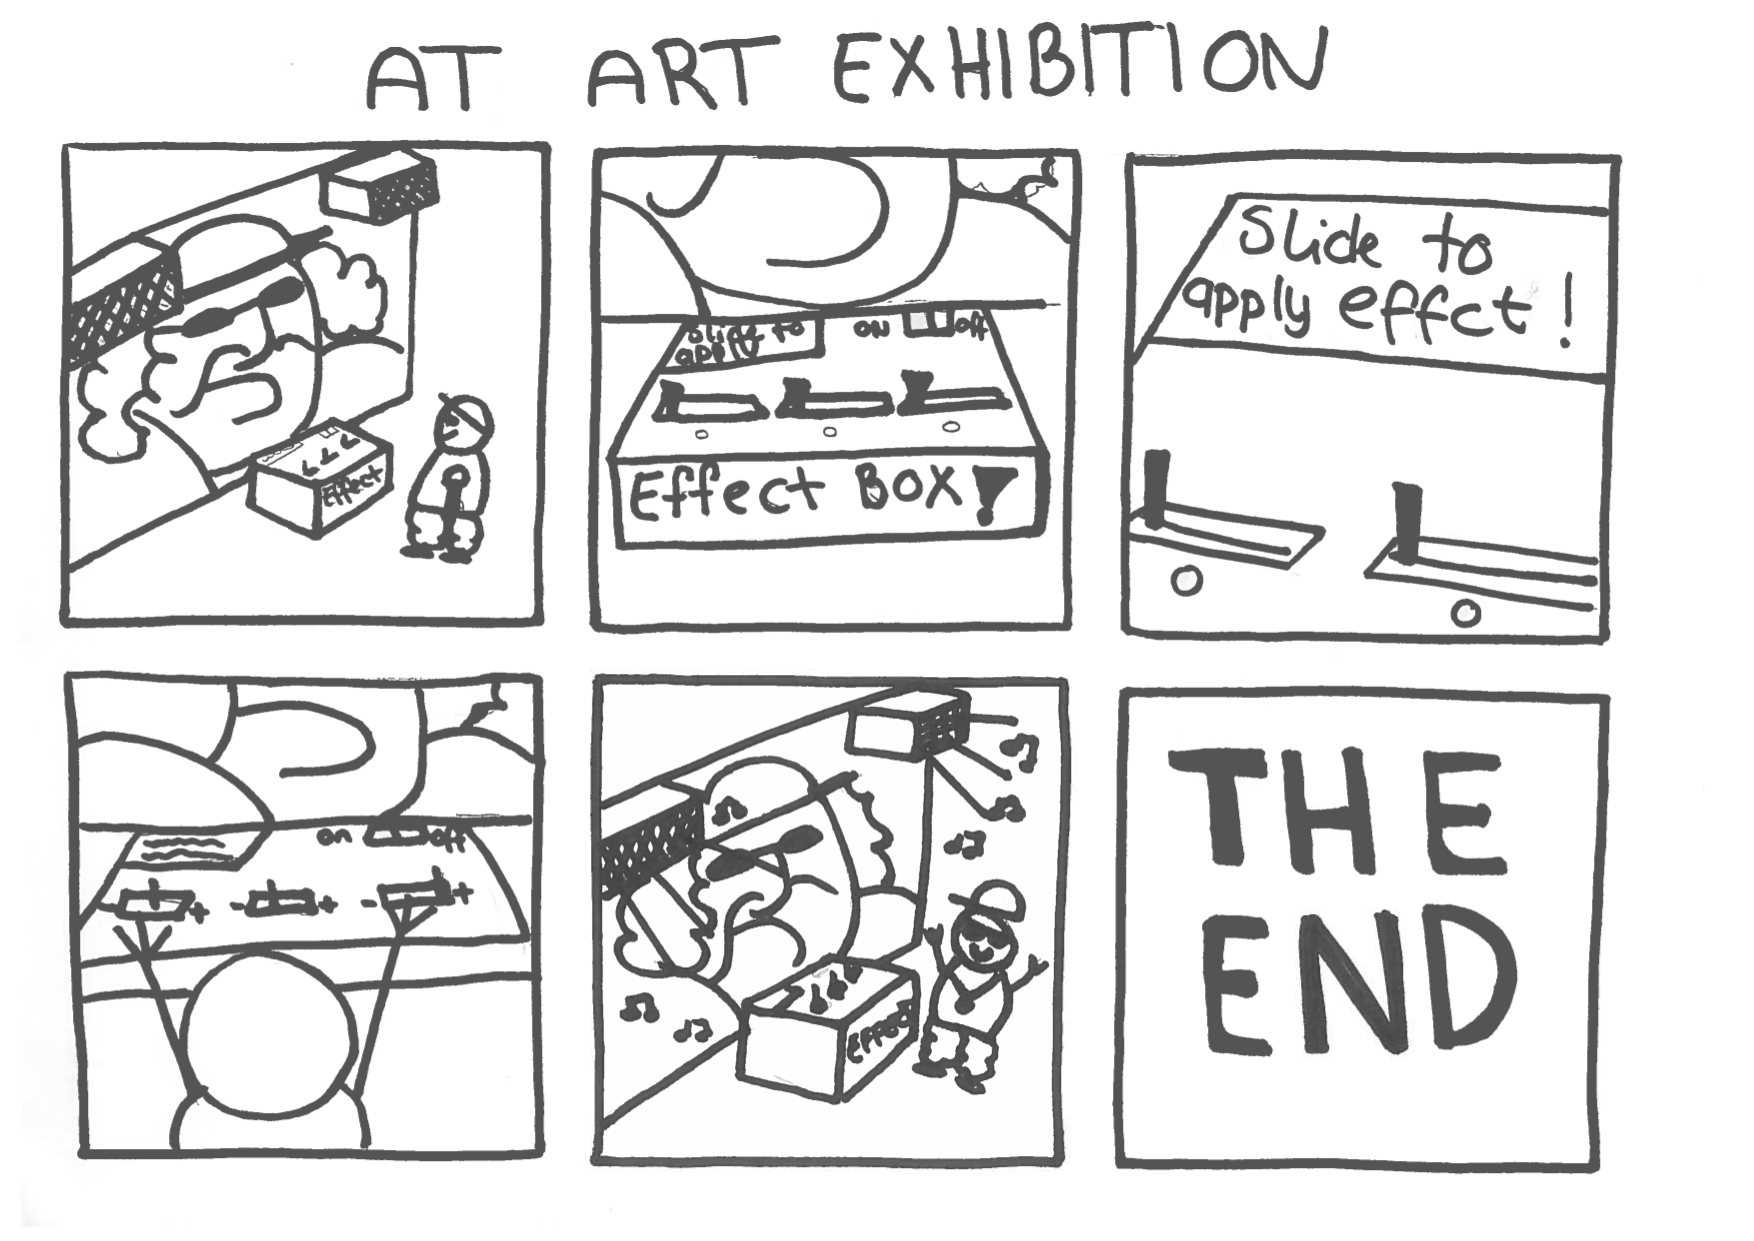
\includegraphics[width=1\textwidth]{Flowdiagram}
\caption{\label{fig:Flowdiagram} }
\end{figure}

\section{Peripheral devices}
The user has to be able to affect the audio the image generates by interacting with a physical interface. The system will apply an effect which can be modified through a physical device which changes the variable range of the power of the effect from 0\% to 100\%, or in numbers 0 to 1. For this interface these different variations of a peripheral devices has been considered: 

\begin{itemize}
\item Button
\item Pressure sensor
\item Ultra sonic distance sensor
\item Potentiometer
\item Slider
\item Bend sensor
\end{itemize}

Each of these peripheral devices makes the user interact with the prototype differently and changes the functionality of the prototype depending on which peripheral device are implemented.
The button's functionality is it can be clicked. The button have two states: low and high. The low state is when the button is not clicked, and the high state is when the button is being clicked. This means that a system using a button will have programmed states, which will be cycled through in a predetermined or random direction.
Variable resistors allow a system to have a position between the two extremes of low and high. This allows the system to have more fluent control than a simple binary choice of on or off. There are multiple variable resistors to choose from, which changes the user's interaction with the given device depending on the used peripheral device.  They all function in a fundamentally similar way. 
Pressure sensors react to being pressured, such as from touching and pushing. More pressure equals to a higher position on the scale.
Ultra sonic distance sensors measures the distance between the sensor and a surface in front of the sensor by sending out pulses. The further away the sensor is from an object, the more frequent it will send out a pulse until the echo returns to the sensor. 
Potentiometers can adjust between a minimum and maximum position. Depending on how much the potentiometer is turned it will result in the scale output from the device. Turning knobs is an example of potentiometers. A slider is a variant of a potentiometer with a linear interface instead of a rotary one.
Unlike the previously mentioned variable resistors that all have a clear low and high state, the bend sensor functions differently. The bend sensor rests at a mid-point between low and high. Depending on which direction the sensor is bent the resistance will either go up or down.
These devices would be used as a variable controller for the different effects. Depending on which device is chosen, the integration for the user will be different. This will be tested in the iterations of the prototype and discussed further to make sure that the interface is user-friendly and easy to understand. 

\todo{expand upon the advantages and disadvantages of the different categories of devices}


\section{Electrical Component Test}
Since multiple components were available, a test had to be conducted in order to choose the most preferred and intuitive to use. All the previous mentioned electronic components were used in the test, though there was two different buttons and 3 different potentiometers. All the different components can can be seen on figure \ref{fig:komponenter}. These components were all mounted on a cardboard plate as seen on figure \ref{fig:componenttest}.

\begin{figure}[!h] 
\centering
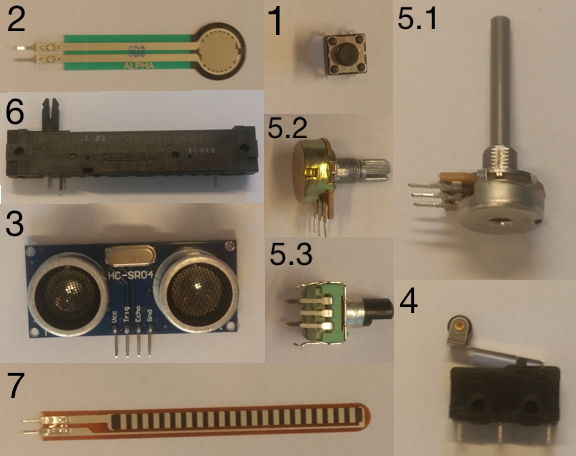
\includegraphics[width=1\textwidth]{komponenter}
\caption{\label{fig:komponenter} The 9 different components used in the test: 1. Normal push button, 2. Pressure sensor, 3. Ultrasonic distance sensor, Telegraph button, 5.1. and 5.2. and 5.3. are the different potentiometers, 7. Bend sensor.}
\end{figure}

\begin{figure}[!h] 
\centering
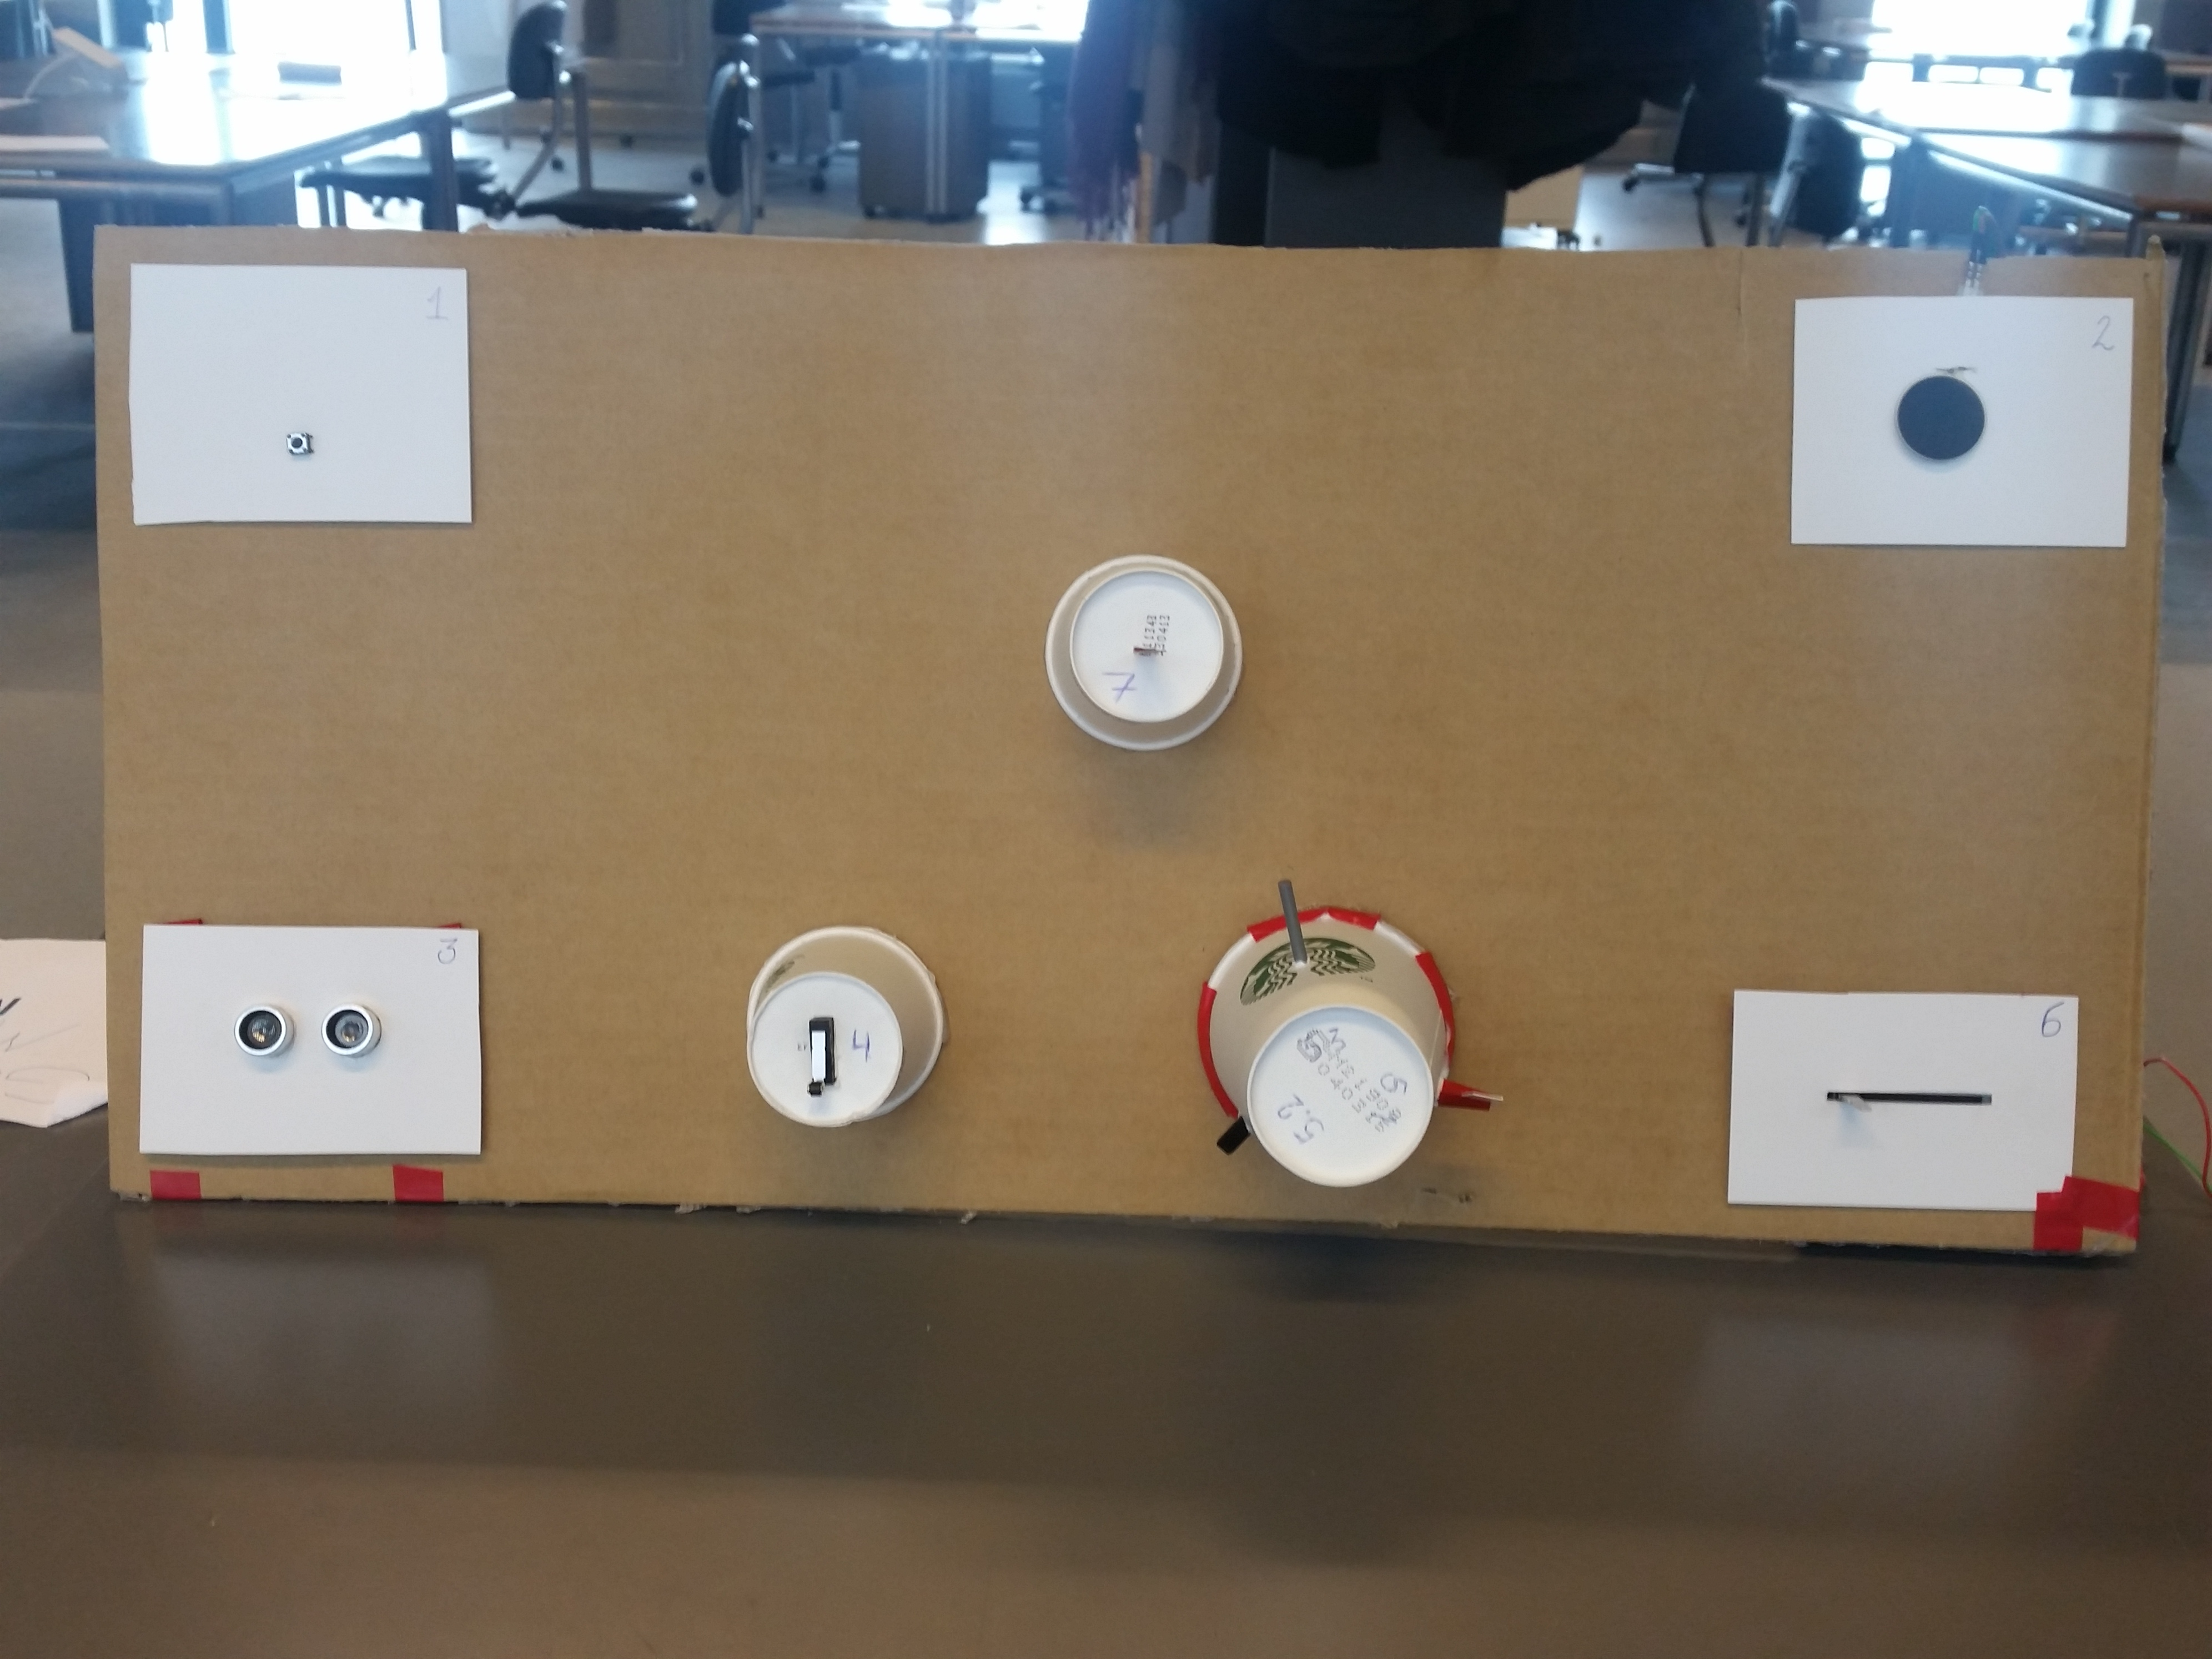
\includegraphics[width=1\textwidth]{componenttest}
\caption{\label{fig:componenttest} The component board used in the component test used to determine which electrical component to use.}
\end{figure}

The test was conducted on 10 participants, all fellow students from Medialogy. The participants were explained by "Test Facilitator 1" how each component worked and how to interact with them. They were told that they had to use all of the components one at a time in a numeral order and think out loud when using the components. "Test Facilitator 2" turned the volume of the music up and down, corresponding to how much the participant !!turned/clicked/slid/moved their hand!!.

Results, as can be seen on figure \todo{indsæt skema over resultater} showed the participants preferred using the slider when changing the volume of the music. A new design sketch was created based on this result.


\section{The chosen sketch}
Based on feedback from the components test, an interface design sketch were made to make a paper mock-up test, the sketch can be seen on figure \ref{fig:sketchmock}. 

\begin{figure}[!h] 
\centering
\includegraphics[width=1\textwidth]{sektchmock}
\caption{\label{fig:sketchmock} Sketch showing the chosen interface for a paper mock-up test.}
\end{figure}

The chosen sketch consists of an on/off button, two sliders with two different effects and a button that changes the state of the effects so that when the device is turned on, the device automatically goes into state one, which is "Effect 1" is turned on. When the user presses the button once, the device goes into state two, which means that "Effect 1" turns off and "Effect 2" turns on. When the users presses the button for the third time, the device goes into state three, which means that both "Effect 1" and "Effect 2" is turned on at the same time, if the user presses the button again the circut starts all over again with state one. If the user grabs one of the sliders and moves it from side to side the effects will change intensity, this works in every single state. When the user is done, he/she simply turns off the device by pressing "off". 

\section{Interface low-fi test}
The chosen sketch was made into a paper mock-up to test the \todo{ind i glossary med dig} percieved affordance and the \todo{dette kan betyde forskellige ting i forskellige sammenhænge} feedforward. Since it was a paper mock-up, no electronic components were used. What should have been the audio feedback was replaced with an drawing of a light bulb in order for understanding the intention of changing the intensity of an object. The paper mock-up can be seen on figure \ref{fig:Papermockoff}.

\begin{figure}[!h] 
\centering
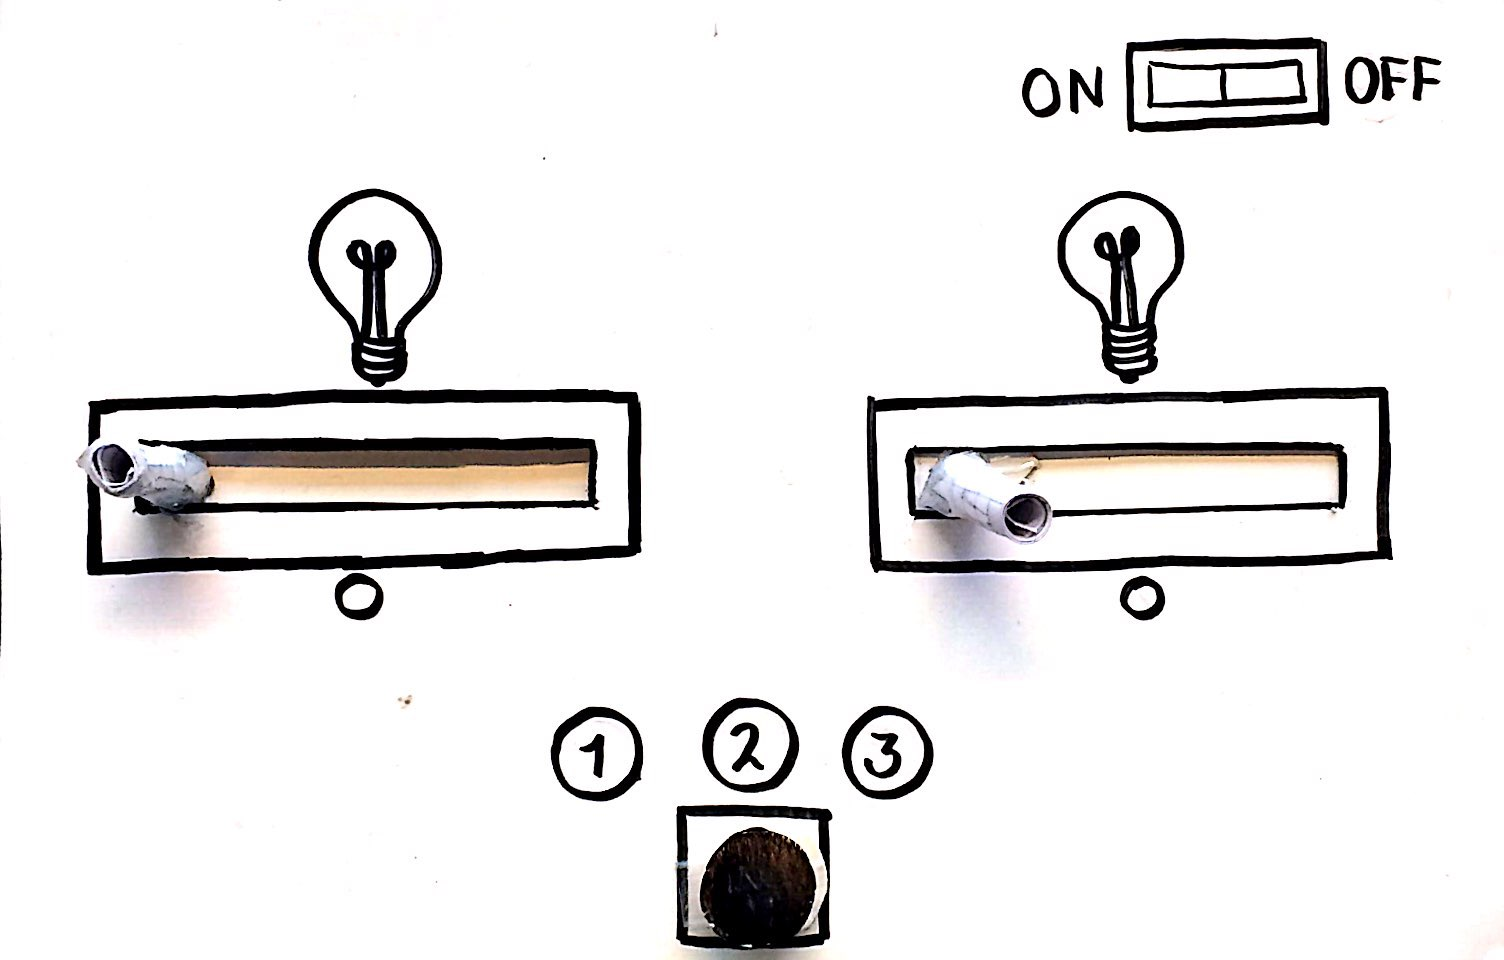
\includegraphics[width=1\textwidth]{Papermockoff}
\caption{\label{fig:Papermockoff} shows the low-fi paper mock-up of interface.}
\end{figure}

The mock-up was tested on 6 fellow Medialogy students. "Test Facilitator 1" explained how the interface works and asked the participant to execute the following tasks:

\begin{itemize}
\item Turn on the device
\item Turn on slider 1
\item Change the intensity of the illumination of light bulb 1
\item Turn on slider 2
\item Change the intensity of the illumination of light bulb 2
\item Turn on both sliders
\item Change the intensity of both or individually both light bulbs
\item Turn off the device
\end{itemize}

\todo{beskrive neutrale states}

Results showed that it was clear that to the user that he/she had to use the slider to change the intensity of the light bulb. However, switching between the states of which slider was in use, proved to be difficult for the user since their perception the feedforward was not clear enough. Some users suggested the use of imagery for better understanding of the interface.
Since the feedforward of the slider was not sufficient enough, a feedforward test was conducted.

\section{Feedforward test}
Eight different designs for the slider was made, as can be seen on the figure below.

\begin{figure}[!h] 
\centering
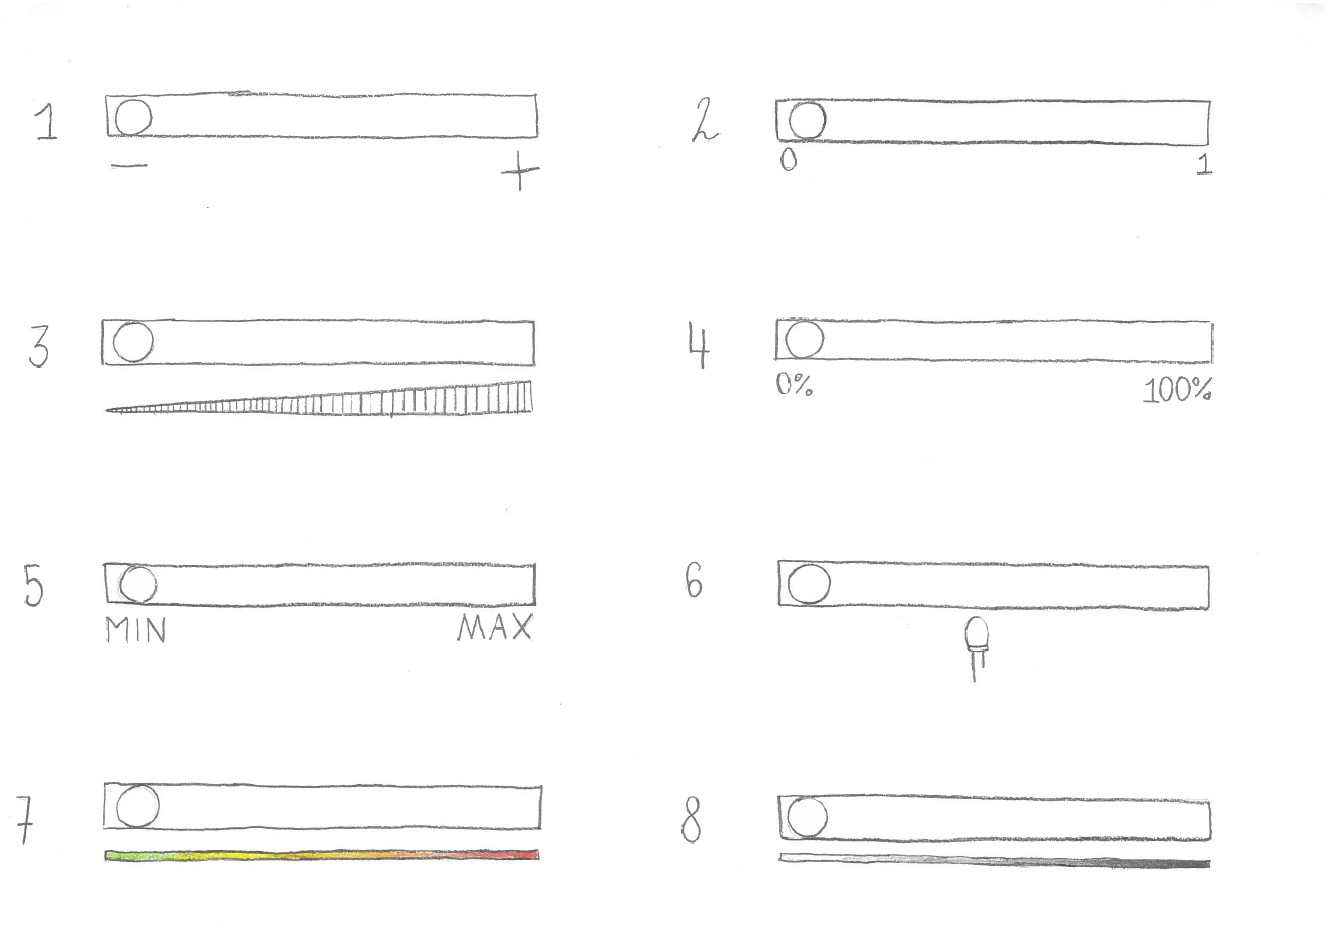
\includegraphics[width=1\textwidth]{fftestimage}
\caption{\label{fig:fftestimage} The 8 different designs for the feedforward test.}
\end{figure}

The participants for this test were also from the Medialogy studies. The test included 46 participants. The participants were explained the context of use !for the slider! and after asked to choose one of the eight different designs that they thought had the best feedforward. The participants were all sitting in their group areas, so to ensure the participants answers were not affect each others, they were asked to point at a piece of paper with numbers, representing the different designs, randomly located on the paper to further ensure confidentiality when telling the test facilitator what their answers were. 

!insert figure with numbers of answers!

Statistically speaking, the most preferred feedforward design was the fifth design with "MIN" and "MAX" written on it had 15 votes while the third feedforward design with the "Amplitude Bar" \todo{definer} received 14 votes. The fourth design with the values "0\%" percent "100\%" percent had the third highest amount of votes being nine out of 46 and the least favourite designs were the seventh with 3 votes and the first and second design with 2 votes each and the sixth design with only one vote. 

\begin{table}[!h]
\centering
\caption{Shows the results of the feedforward test.\label{tab:sliderresults}}
\begin{tabular}{|l|c|c|c|c|c|c|c|c|}
\hline
Design & 1 & 2 & 3 & 4 & 5 & 6 & 7 & 8 \\ \hline
Amount of votes & 2 & 2 & 14 & 9 & 15 & 1 & 3 & 0 \\ \hline
\end{tabular}
\end{table}

As can be seen on table \ref{tab:sliderresults}, the most preferred feedforward design was design five that had 15 votes while the design three received 14 votes and design four had nine votes.
Even though the third and fifth feedforward design received almost the same amount of votes, the design team choose to go with the fifth design. The prototype will be expanded of this design and it will be taken into further iterations of the performance testing. 


\section{Final design sketches}
This section shows and describes the final interface design

\begin{figure}[!h] 
\centering
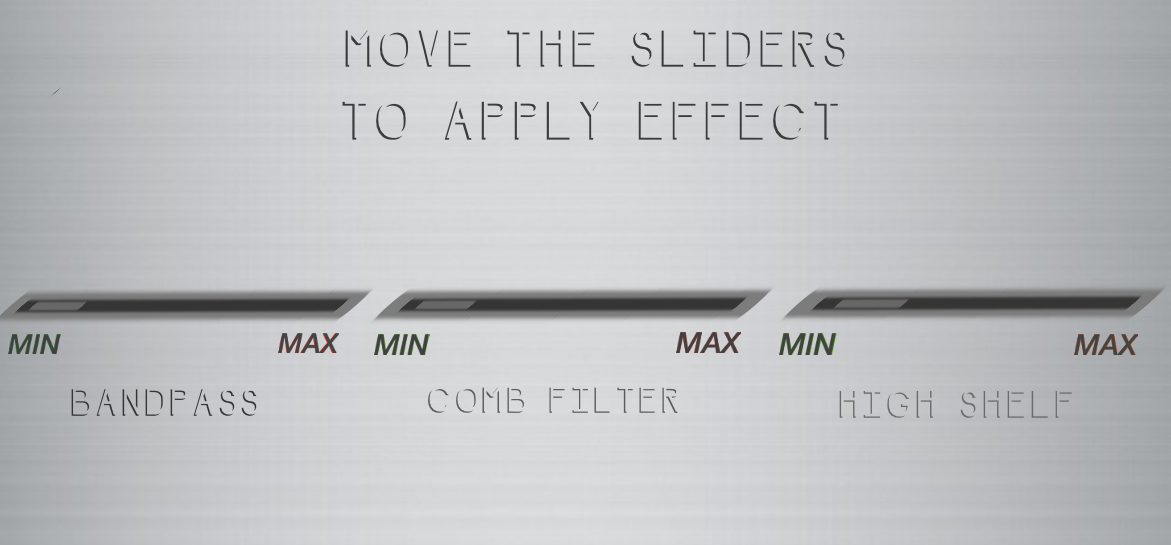
\includegraphics[width=1\textwidth]{finaldesignsketch3grey}
\caption{\label{fig:inaldesignsketch3grey} The figure shows a sketch of the final interface design made by elaborate on the former sketches and feedback from the users during tests .}
\end{figure}

\section{Final design sketches}
\begin{figure}[!h] 
\centering
\includegraphics[width=1\textwidth]{finalinterfacewood}
\caption{\label{fig:finalinterfacewood} This figure also shows the final interface design but in a wood variation .}
\end{figure}
 
 
 The final interface design is based on test result from our previous sketches and component tests. The final interface is 
 
 
 
 \section{Final product }
*indsæt billeder af den færdigbyggede kasse* 

The finished product is build based on the sketches figure xx* The product is made of wood and is kept in neutral colours so the user / owner / museum is to determine the colour of the box so it matches the specific art work as show in in *figure xxx - billede af seupet med farve på* To reach the optimal hight of the box, it will be places on a stander / pedistal / something. 








